\documentclass[a4paper,runningheads]{llncs}
\usepackage[T1]{fontenc}
\usepackage{graphicx}
\usepackage{booktabs}
\usepackage{amsmath,amssymb}
\usepackage{microtype}
\usepackage{url}
\usepackage{cite}

\InputIfFileExists{generated/macros.tex}{}{}
\InputIfFileExists{generated/macros_review.tex}{}{}
\providecommand{\PermMaxCarf}{??}\providecommand{\NPerm}{??}\providecommand{\PermPCarf}{??}\providecommand{\PermMeanCarf}{??}
\newcommand{\logit}{\operatorname{logit}}

\pdfinfoomitdate=1
\pdftrailerid{}
\pdfsuppressptexinfo=-1
\begin{document}
\title{Supplementary Material:\\ CARF: Bounded Anchored Fusion for Multimodal Prediction with Unreliable Modalities}
\titlerunning{CARF: Bounded Anchored Fusion (Supplement)}
\author{Sachin Kumar\inst{1}\orcidID{0009-0007-2893-0655} \and
Subhankar Mishra\inst{1}\orcidID{0000-0002-9910-7291}}

\institute{School of Computer Sciences, National Institute of Science Education and Research (NISER), Bhubaneswar, India\\
\email{smishra@niser.ac.in}}
\maketitle

\setcounter{section}{0}
\renewcommand{\thesection}{S\arabic{section}}
\renewcommand{\thetable}{S\arabic{table}}
\renewcommand{\thefigure}{S\arabic{figure}}

\section{Data and preprocessing}

\paragraph{Patient linkage.} Identifiers are matched explicitly across the clinical, expression, imaging, and RPPA sources. The development cohort contains \NDev{} I-SPY2 patients (\NDevPos{} with pCR) with clinical data, expression (GSE194040), and usable pretreatment MRI; RPPA \cite{wolf2022ispy} is available for \NRppa{} of them (\NRppaFeat{} features). The external cohort contains \NExt{} I-SPY1 patients (\NExtPos{} with pCR) with expression (GSE22226) and usable MRI and no RPPA. Expression is restricted to the \NGenes{} shared genes and replaced, for each patient, by within-patient ranks divided by the number of observed genes; missing values are imputed with the training median inside every expert fit.

\paragraph{Treatment-aware anchor.} The anchor is a class-balanced logistic regression ($C=1$) on age, HR status, HER2 status, and four therapy-class indicators derived from the assigned regimen: anti-HER2 antibody (trastuzumab, pertuzumab, or T-DM1), immunotherapy (pembrolizumab), platinum (carboplatin), and HER2 tyrosine-kinase inhibitor (neratinib). In I-SPY1, all patients received anthracycline-based chemotherapy, and the anti-HER2 indicator is set from the recorded regimen (AC+T+trastuzumab); I-SPY1 patients without an expression record (natural-missingness analysis) and GSE25066 patients are assigned no anti-HER2 therapy. The therapy class is fixed before treatment starts and is therefore a legitimate input of a pretreatment prediction under a planned regimen. In a preliminary internal check, subtype-by-therapy interactions did not improve the anchor and were not used.

\paragraph{Experts and auxiliary heads.} RNA: training-median imputation, top 3{,}000 genes by training variance, 250 genes by ANOVA $F$-test, standardization, logistic regression with $C=0.1$. MRI: \NMriFeat{} fixed features (54 signal summaries of the precontrast, early, and late phases and enhancement maps, six shape descriptors, two kinetic fractions, four texture descriptors), median imputation, standardization, $C=1$. RPPA: median imputation, standardization, $C=0.01$; fitted and applied only on patients with RPPA. The auxiliary heads use the same preprocessing (50 ANOVA-selected genes for RNA) and unweighted logistic regressions for HR and HER2 status, fitted on training patients with recorded values. Larger RNA gene sets were screened during development; because I-SPY1 performance informed their rejection, the I-SPY1 results are exploratory rather than an untouched validation.

\paragraph{Verification gate.} For modality $j$ and a patient with recorded HR/HER2 values $c=(c_1,c_2)$, the auxiliary heads give $q_{jt}$, and $\ell_j=\prod_t q_{jt}^{c_t}(1-q_{jt})^{1-c_t}$. The swap likelihood $\bar\ell_j=\frac1N\sum_{i}\prod_t q_{ijt}^{c_t}(1-q_{ijt})^{1-c_t}$ averages over the inner out-of-fold auxiliary predictions $q_{ij}$ of the $N$ training patients with modality $j$, i.e., it is the likelihood of the record if the sample came from a random training patient. The gate $g_j=\pi\ell_j/(\pi\ell_j+(1-\pi)\bar\ell_j)$ with $\pi=0.95$ is a posterior probability in $[0,1]$. In the swap environments of the objective and in the swap stress tests, the auxiliary predictions move with the swapped sample and the gate is recomputed against the receiving patient's record. Pooled over the internal test folds, the gate separates own from swapped samples with AUROC \GateAucRna{} (RNA), \GateAucRppa{} (RPPA), and \GateAucMri{} (MRI); own samples have a gate below 0.5 in \GateLowTrueRna\% (RNA) and \GateLowTrueRppa\% (RPPA) of the cases.

\paragraph{Gated baselines and mix-ups.} Each gated baseline is the corresponding baseline fitted to $\tilde p_j=\sigma(a+g_j(\logit p_j-a))$, where $g_j$ is the verification gate with the training patients' out-of-fold auxiliary predictions as reference, exactly as in CARF; missing experts stay missing. The semi-realistic mix-ups affect RNA and RPPA. \emph{Offset}: the patients with the modality are ordered by GEO accession number, and a contiguous run of 20\% of them (random start) receives the sample of the preceding patient. \emph{Batch}: 20\% of the samples are drawn at random and permuted among themselves within their processing batch (I-SPY2 expression: array platform and normalization method; RPPA: array; I-SPY1: one batch). \emph{Subtype}: all samples are permuted within the three HR/HER2 subtypes. In every mix-up, the auxiliary predictions move with the sample.

\section{Full comparison tables}

Table~\ref{tab:ci} reports paired intervals for the failure average and the worst case of CARF against every comparator. Table~\ref{tab:stress} reports the main failure scenarios, Table~\ref{tab:design} the effect of the anchor and of RPPA, Table~\ref{tab:ablation} the CARF ablations, Table~\ref{tab:internalfull} all internal failure scenarios, Table~\ref{tab:externalfull} all external output-level scenarios, including the extreme and neutral outputs used in training, and Table~\ref{tab:inputfull} all input-level corruption levels. Fig.~\ref{fig:tradeoff} summarizes the trade-off between accuracy on intact inputs and in the worst failure scenario.

\begin{table}[h]
\centering
\caption{CARF minus comparator, failure-average and worst-case AUROC: point estimate and 95\% interval (internal: corrected resampled $t$ over 25 folds; external: 2{,}000 paired patient bootstrap resamples with realizations held fixed). Positive values favor CARF.}
\label{tab:ci}
\setlength{\tabcolsep}{3pt}
\resizebox{\linewidth}{!}{\InputIfFileExists{generated/tab_supp_ci.tex}{}{}}
\end{table}

\begin{table}[h]
\centering
\caption{AUROC under failure of one optional modality (sw.: sample swap; miss.: removed). Internal: mean over 25 folds with 5 realizations each ($n=\NDev$). External: mean of 30 realizations ($n=\NExt$); input-level corruptions are applied to the inputs of the frozen experts. Bold: best fusion model.}
\label{tab:stress}
\setlength{\tabcolsep}{3pt}
\resizebox{\linewidth}{!}{\InputIfFileExists{generated/tab_stress.tex}{}{}}
\end{table}

\begin{table}[h]
\centering
\caption{Effect of the anchor and of the partially available modality. Internal AUROC on intact inputs (mean over 25 folds) for four designs, and internal RNA-swap AUROC and failure average of CARF. Bold: best model per design.}
\label{tab:design}
\setlength{\tabcolsep}{3pt}
\resizebox{\linewidth}{!}{\InputIfFileExists{generated/tab_design.tex}{}{}}
\end{table}

\begin{figure}[h]
\centering
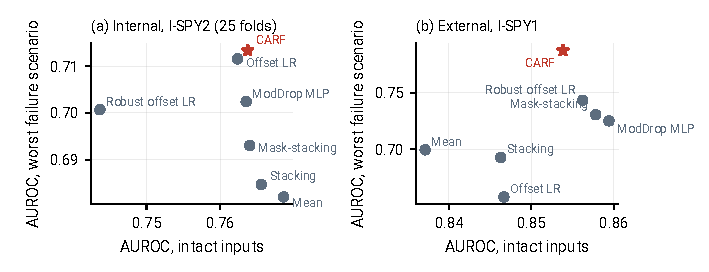
\includegraphics[width=0.9\linewidth]{figures/fig_tradeoff.pdf}
\caption{AUROC on intact inputs versus AUROC in the worst failure scenario, (a) internally and (b) externally.}
\label{fig:tradeoff}
\end{figure}

\begin{table}[h]
\centering
\caption{Ablation of CARF components (treatment-aware anchor, RNA, MRI, and RPPA).}
\label{tab:ablation}
\small
\InputIfFileExists{generated/tab_ablation.tex}{}{}
\end{table}

\paragraph{Budget sensitivity.} Inner cross-validation selects $B=1.5$ or $2$ (\BudgetList{} of 25 folds). A fixed $B=1$ gives similar external RNA-swap robustness (\ExtRnaSwapCarfTwoBOne{}) at a lower internal accuracy (\IntCarfTwoBOne{}); training without swaps in the objective gives a comparable external RNA-swap AUROC (\ExtRnaSwapCarfTwoNoSwap{}) and internal accuracy (\IntCarfTwoNoSwap{}), so the swap environments in Eq.~2 of the main paper are not the main source of robustness, the clipped budget is. The fully unbounded rule, which removes the clip and the budget constraint, carries no displacement guarantee and reaches a maximum displacement of \MaxDispCarfTwoUnbounded{} logits from the anchor, compared with CARF's bounded \MaxDispCarfTwo{} logits, below the sharp budget of the RNA and MRI terms (\SharpBudgetExt{}); other fusion models, gated or not, move predictions by up to \MaxDispGatedOffsetLr{} logits.

\paragraph{Fallback.} To quantify the contribution of the fallback mechanism separately from the bound and the gate, the \emph{all-missing} scenario (every optional modality absent) of Tables~\ref{tab:internalfull} and \ref{tab:externalfull} isolates it directly: by construction every term of Eq.~1 of the main paper is zero when every $m_j=0$, so CARF, carf2\_no\_gate, and every other CARF ablation reproduce the clinical model's AUROC and Brier score \emph{exactly} (max.\ displacement $<10^{-15}$, i.e., floating-point zero, internally and externally), whereas every baseline without an exact fallback moves the prediction away from the anchor (external max.\ displacement: mask-stacking 0.649, offset LR 0.710, robust offset LR 0.728, stacking 0.834, ModDrop MLP 1.273 logits), even though AUROC is unaffected in this cohort because the shift is a near-constant offset that does not change the ranking. The exact fallback is therefore not merely a convenience: it is what makes ``no optional data available'' auditable as \emph{identical} to the clinical-only prediction, rather than merely similar to it, and this identity is a free consequence of the bound and does not depend on $B$, $\theta$, or the gate -- disabling either of the latter two (carf2\_no\_gate, carf2\_unbounded in Table~\ref{tab:ablation}) leaves the fallback property untouched. This exactness is not automatically the best-calibrated choice in this one scenario: offset LR and robust offset LR have a learned global intercept that happens to give a marginally lower external Brier score under all-missing (0.157 and 0.157 vs.\ CARF's 0.185, both using the same class-balanced clinical expert), illustrating a genuine trade-off between an exact, verifiable identity and the best possible fallback calibration.

\begin{table}[h]
\centering
\caption{Internal AUROC (I-SPY2, mean over 25 folds; swap: 5 realizations per fold) for all scenarios.}
\label{tab:internalfull}
\scriptsize
\setlength{\tabcolsep}{3pt}
\resizebox{\linewidth}{!}{\InputIfFileExists{generated/tab_supp_internal.tex}{}{}}
\end{table}

\begin{table}[h]
\centering
\caption{External AUROC (I-SPY1) for all output-level scenarios (swap and noisy: mean of 30 realizations; noisy: Gaussian noise of SD 0.25 on the probability; low/high/neutral: output set to 0.01/0.99/0.5) and the largest displacement from the anchor over all scenarios. R: RNA; M: MRI.}
\label{tab:externalfull}
\setlength{\tabcolsep}{2pt}
\resizebox{\linewidth}{!}{\InputIfFileExists{generated/tab_supp_external.tex}{}{}}
\end{table}

\begin{table}[h]
\centering
\caption{External AUROC under input-level corruption of the frozen experts (mean of 30 realizations): fraction of genes removed, fraction of genes shifted by two log-ratio units, Gaussian noise on the MRI features in training SDs, and fraction of MRI features removed.}
\label{tab:inputfull}
\setlength{\tabcolsep}{3pt}
\resizebox{\linewidth}{!}{\InputIfFileExists{generated/tab_supp_input.tex}{}{}}
\end{table}

\paragraph{Statistical tests.} Internal differences use per-fold paired AUROC differences over the 25 outer folds and the corrected resampled $t$-test with test-to-training ratio $1/4$ \cite{nadeau2003}; the per-fold results of all comparisons are written to \texttt{internal\_paired.csv} by the analysis code.

\section{Additional cohort: GSE25066}

We evaluate the I-SPY2-trained pipeline on GSE25066 without its I-SPY1 samples. For feature compatibility, the RNA expert is refitted on I-SPY2 using only genes shared with GSE25066; no labels from the new cohort are used. MRI and RPPA are absent for all patients. Table~\ref{tab:gse} reports the results.

\begin{table}[h]
\centering
\caption{GSE25066 without its I-SPY1 samples (\GseN{} patients, \GsePos{} with pCR; RNA refitted on I-SPY2 restricted to the shared genes; MRI and RPPA absent). Swap and dropout: mean of 30 realizations.}
\label{tab:gse}
\small
\InputIfFileExists{generated/tab_supp_gse.tex}{}{}
\end{table}

\section{Third external cohort: GSE20194 (MAQC-II BR / MDACC)}

As a larger, independent validation cohort not used for feature selection, GSE20194 (MAQC-II BR, MDACC, Affymetrix U133A, pCR vs.\ residual disease) is a third, previously unused external cohort of \GseTwoZeroOneNineFourN{} patients (\GseTwoZeroOneNineFourPos{} with pCR; no MRI, no RPPA), evaluated with the frozen experts and fusions of CARF v1 ($B=1$, $\gamma=0.25$; this cohort predates CARF-2's RPPA modality and treatment-aware anchor, which this cohort cannot use anyway since it has neither RPPA nor treatment-regimen metadata). As with GSE25066, the RNA expert is refit on I-SPY2 restricted to shared genes, and no GSE20194 label is used for any fitting step.

\emph{This is not a fully independent cohort.} \GseTwoZeroOneNineFourOverlapN{}/\GseTwoZeroOneNineFourN{} GSE20194 patients (81\%) share a patient identifier with GSE25066's MDACC source and are confirmed as near-identical arrays (array correlation $\ge 0.99$ for matched pairs, perfect clinical-field agreement); only \GseTwoZeroOneNineFourUniqueN{} patients (\GseTwoZeroOneNineFourUniquePos{} with pCR) are unique to GSE20194. We therefore report the full cohort for comparability with the pre-existing analysis that produced these numbers, and the unique subset, descriptively, as the only genuinely new validation it provides.

\begin{table}[h]
\centering
\caption{GSE20194 (230 patients, 48 pCR; RNA refit on I-SPY2 restricted to shared genes; MRI and RPPA absent), CARF v1.}
\label{tab:gse20194}
\small
\InputIfFileExists{generated/tab_gse20194.tex}{}{}
\end{table}

On intact inputs, CARF (\GseTwoZeroOneNineFourCarf{}, 95\% CI $[\GseTwoZeroOneNineFourCarfLo{},\GseTwoZeroOneNineFourCarfHi{}]$) is indistinguishable from the clinical model (\GseTwoZeroOneNineFourClinical{}) and from stacking (\GseTwoZeroOneNineFourStack{}); no fusion model beats the clinical anchor on this cohort, consistent with a weak cross-platform RNA expert here (Agilent-trained, applied to Affymetrix U133A). Under 50\% per-patient gene dropout, CARF (\GseTwoZeroOneNineFourDropoutCarf{}) again loses far less than stacking (\GseTwoZeroOneNineFourDropoutStack{}) or the clinical model alone would suggest is possible to preserve (\GseTwoZeroOneNineFourDropoutClinical{}), reproducing the robustness pattern of the main cohorts on an entirely different RNA platform. On the \GseTwoZeroOneNineFourUniqueN{}-patient subset that is not also in GSE25066, the numbers are close and descriptive only given the small size (CARF \GseTwoZeroOneNineFourUniqueCarf{}, clinical \GseTwoZeroOneNineFourUniqueClinical{}, stacking \GseTwoZeroOneNineFourUniqueStack{}). Taken together with GSE25066 (Sec.~S3), this gives two independent-platform external cohorts beyond I-SPY1 (409 and 230 patients, 81\% overlapping with each other and 0\% with I-SPY1 or I-SPY2), which extends independent-cohort validation without fully resolving the need for a larger one: both lack MRI and RPPA, so they cannot test the multi-modal or anchor-failure claims, and the only cohort unique to GSE20194 is too small (44 patients) to be more than descriptive.

\section{Naturally missing modalities}

Table~\ref{tab:natural} reports the full results for the I-SPY1 patients with naturally missing modalities discussed in the main paper.

\begin{table}[h]
\centering
\caption{I-SPY1 patients with their true availability masks (columns: subset, number of patients/with pCR). ``all'' contains every patient with at least one optional modality; ``partial'' contains patients with exactly one.}
\label{tab:natural}
\setlength{\tabcolsep}{3pt}
\resizebox{\linewidth}{!}{\InputIfFileExists{generated/tab_supp_natural.tex}{}{}}
\end{table}

\section{Calibration}

All experts use class-balanced weights, so all models overestimate the prevalence. Table~\ref{tab:calib} reports calibration on intact inputs with no recalibration, as in our original submission.

\begin{table}[h]
\centering
\caption{Calibration on intact inputs, no recalibration (lower is better).}
\label{tab:calib}
\small
\InputIfFileExists{generated/tab_supp_calib.tex}{}{}
\end{table}

\paragraph{Post-hoc recalibration.} To correct this overestimation, we fit Platt scaling, a one-dimensional logistic regression of the label on the logit of each model's probability, $\sigma(\alpha\,\logit p+\beta)$, which cannot change AUROC or the bound of Sec.~3.2 since it is a monotone affine map of the logit. Internally, $(\alpha,\beta)$ is fit and applied by five-fold cross-validation of the pooled out-of-fold predictions underlying Table~1 of the main paper, so the reported internal numbers are themselves out-of-sample. Externally, $(\alpha,\beta)$ is fit once on all pooled internal out-of-fold predictions and applied to the external cohort; no external label is used to fit it. Table~\ref{tab:calib-review} reports Brier score, expected calibration error, and predicted versus observed prevalence before and after, for every model. Recalibration closes most of the prevalence gap for every model that used class-balanced weights (e.g., CARF: \CalibExtCarfPrevBefore{}$\to$\CalibExtCarfPrevAfter{} predicted vs.\ \CalibTruePrev{} observed externally) and improves Brier score and ECE for CARF, stacking, and mask-stacking; offset LR, robust offset LR, and ModDrop MLP were already close to calibrated, since their unweighted or near-unweighted intercepts partially absorb the class-balancing offset, and recalibration changes them little.

\begin{table}[h]
\centering
\caption{Calibration before$\to$after Platt recalibration (lower Brier/ECE is better; predicted prevalence should match the observed \CalibTruePrev{} externally, \GsePos{}/\GseN{} internally -- see Table~\ref{tab:calib}).}
\label{tab:calib-review}
\scriptsize
\setlength{\tabcolsep}{3pt}
\resizebox{\linewidth}{!}{\InputIfFileExists{generated/tab_calib_review.tex}{}{}}
\end{table}

\paragraph{Decision-curve analysis.} Using the externally recalibrated probabilities, we compute net benefit $\mathrm{NB}(p_t)=\mathrm{TP}/n-(\mathrm{FP}/n)\,p_t/(1-p_t)$ over threshold probabilities $p_t\in[0.05,0.5]$, against treat-all and treat-none references, for the clinical model, CARF, and stacking (Fig.~\ref{fig:dc}), a measure of clinical usefulness beyond AUROC: net benefit asks, for a given threshold at which a clinician would act on the predicted probability (e.g., omit or add a therapy), how many correct decisions a model buys per patient relative to treating everyone or no one at that threshold. CARF's net benefit is at or above the clinical model's at every threshold we tried (0.05--0.50), whereas stacking's net benefit falls below the clinical model's from a threshold of 0.35 upward.

\begin{figure}[h]
\centering
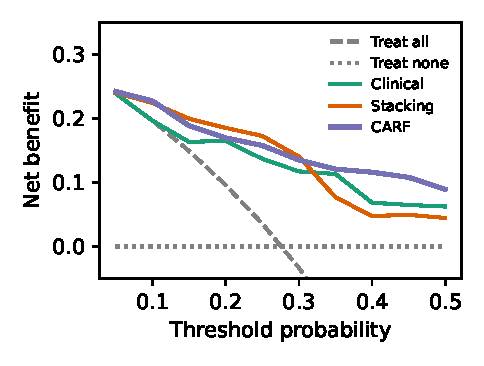
\includegraphics[width=0.62\linewidth]{figures/fig_decision_curve.pdf}
\caption{Decision-curve analysis on the external cohort with Platt-recalibrated probabilities: net benefit of treating as pCR-predicted above each threshold, against treat-all/treat-none references.}
\label{fig:dc}
\end{figure}

\section{Simultaneous modality failures}

Beyond the one-at-a-time failures of Table~\ref{tab:stress}, we consider more realistic corruption scenarios in which multiple modalities fail at once. Using the frozen external models of the main design, we evaluate three combinations, each with 30 realizations: an RNA sample swap together with MRI output noise (Gaussian noise on the probability, SD 0.25, as in Table~\ref{tab:externalfull}); an RNA sample swap together with an independently drawn MRI sample swap; and RNA gene dropout (50\% of genes missing) together with MRI feature dropout (60\% of features missing). Table~\ref{tab:combo-review} reports the full comparison. CARF's margin over the best unbounded baseline (robust offset LR) widens under joint output-level failure relative to either failure alone, consistent with the per-modality budget $b_j$ bounding each failure's contribution additively (Sec.~3.2 of the main paper): an unbounded model's errors can compound across modalities, while CARF's cannot exceed the sum of the per-modality budgets. Under joint input-level dropout, where little signal remains in either modality regardless of the fusion rule, the gap between CARF and robust offset LR is smaller and its interval includes zero.

\begin{table}[h]
\centering
\caption{AUROC under simultaneous modality failures, external cohort (30 realizations each). R: RNA; M: MRI. Bold: best fusion model per row.}
\label{tab:combo-review}
\setlength{\tabcolsep}{3pt}
\resizebox{\linewidth}{!}{\InputIfFileExists{generated/tab_combo.tex}{}{}}
\end{table}

\section{Anchor failure}

CARF bounds the influence of the \emph{optional} modalities relative to the clinical anchor; it carries no guarantee if the anchor itself is wrong. We simulate charting error directly: for a random subset of external patients, we flip the recorded HR status, HER2 status, or both, at three error rates (5\%, 10\%, 20\%), with 30 realizations each. This corrupts (i) the anchor logit $a$, since every expert's residual and the anchor column itself are computed from the clinical block, and (ii) the verification gate, since $g_j$ checks each optional sample's auxiliary prediction against this same (now wrong) record, so a genuinely well-matched RNA or MRI sample can look inconsistent purely because the chart is wrong. Table~\ref{tab:anchor-review} reports every model and error level.

Unlike the modality failures elsewhere in this paper, CARF is \emph{less} robust than stacking and most other unbounded baselines under anchor corruption, and the gap grows with the error rate. Comparing CARF with and without its gate isolates the gate's own contribution to this gap: removing the gate recovers roughly half of CARF's loss relative to stacking at the 20\% combined error level (main paper, Sec.~4.2), confirming that the gate, which is only as reliable as the anchor it checks against, actively amplifies anchor error rather than merely failing to help. This is the clearest case in our evaluation where CARF's design assumption (``the anchor is reliable'') is violated and the method suffers for it.

\begin{table}[h]
\centering
\caption{External AUROC when the clinical anchor itself is corrupted (HR/HER2 status flipped for a random subset of patients; 30 realizations per cell). Bold: best fusion model per row.}
\label{tab:anchor-review}
\setlength{\tabcolsep}{3pt}
\resizebox{\linewidth}{!}{\InputIfFileExists{generated/tab_anchor.tex}{}{}}
\end{table}

\section{Exploratory MRI verification using tumor stage}

The verification gate separates true from swapped samples well for RNA and RPPA (AUROC \GateAucRna{} and \GateAucRppa{}) but barely above chance for MRI (\GateAucMri{}), because HR/HER2 status, our only always-recorded cross-check, is weakly reflected in tumor MRI features. To explore whether an alternative cross-check could improve this, we note that I-SPY1's source metadata additionally records pre-chemotherapy clinical tumor size (cm) and T-stage (categorical: $\le2$, $2$--$5$, $>5$\,cm), fields unused elsewhere in this paper and not available in I-SPY2. As an exploratory, I-SPY1-only check, we binarize T-stage as $\ge 3$ (tumor $>5$\,cm) versus not, and fit a five-fold cross-validated logistic regression from the same MRI features used elsewhere in this paper to this label ($\MriTstageN{}$ patients with both an MRI record and a recorded T-stage, $\MriTstagePos{}$ with T-stage 3). The out-of-fold predictions discriminate T-stage well (AUROC \MriTstageDirectAuc{}), confirming that MRI shape and intensity features carry tumor-size information. Building a gate from this signal exactly as in Eq.~2 of the main paper (prior $\pi=0.95$), and evaluating it with the same true-vs.-swapped AUROC used for Fig.~2 of the main paper (true sample likelihood vs.\ 200 random permutations), gives AUROC \MriTstageGateAuc{}, clearly above the HR/HER2-based MRI gate's \GateAucMri{}; the mean gate of true samples is \MriTstageGateTrueMean{}, and \MriTstageGateSwapLow\% of swapped samples fall below 0.5.

This result does not change the main pipeline: T-stage is not recorded in I-SPY2, so an auxiliary head cannot be trained on the development cohort and applied, under cross-fitting, to new patients the way the HR/HER2 heads are. We report it only to show that the weak MRI gate reflects a verification-\emph{variable} problem specific to HR/HER2, not a limit of the gate mechanism itself, and that a cohort recording tumor stage (or another variable MRI predicts well) during model development, not just at evaluation time, could plausibly support a materially better MRI gate.

\section{Whole-pipeline permutation test}

To test whether the external performance could arise from a pipeline which learns nothing from the development labels, we refit the whole pipeline (experts, auxiliary heads, budget selection, and fusion) on \NPerm{} permutations of the I-SPY2 labels and evaluate on I-SPY1 with the true labels. The external CARF AUROCs have mean \PermMeanCarf{} and maximum \PermMaxCarf{}, compared with the observed \ExtCarfTwo{} ($p=\PermPCarf$).

\bibliographystyle{splncs04}
\bibliography{references}
\end{document}
